\documentclass[12pt,a4paper]{article}

\usepackage[a4paper,margin=1in]{geometry}
\usepackage{graphicx}
\usepackage{booktabs}
\usepackage{amsmath,amssymb}
\usepackage{float}
\usepackage{hyperref}
\usepackage{xcolor}
\usepackage{listings}
\usepackage{enumitem}
\usepackage{fancyhdr}
\usepackage{longtable}

\hypersetup{colorlinks=true,linkcolor=blue,urlcolor=blue,citecolor=blue}

\setlength{\headheight}{14.5pt}
\pagestyle{fancy}
\fancyhf{}
\lhead{ICS1512}
\rhead{Machine Learning Algorithms Laboratory}
\cfoot{\thepage}

\lstset{
language=Python,
basicstyle=\ttfamily\small,
numbers=left,
frame=single,
breaklines=true,
showstringspaces=false
}

\begin{document}

\begin{tabular}{|p{4cm}|p{11cm}|}
\hline
Experiment No. & 9 \\ \hline
Experiment Title & Perceptron vs Multilayer Perceptron (A/B Experiment) with Hyperparameter Tuning\footnotemark \\ \hline
Student Name & Sundareswaran R \\ \hline
Register Number & 3122247001048 \\ \hline
Faculty & Dr. Poreddy Ajay Kumar Reddy \\ \hline
Submission Date & 21 September 2026 \\ \hline
\end{tabular}
\footnotetext{\textbf{GitHub Repository: }\url{https://github.com/The-FOOL-00/ML_Lab}}

% ------------------------------------------------------------
\section{Objective}
The aim of this experiment is to compare two classifiers on the English Handwritten Characters dataset. Model A is a single-layer Perceptron Learning Algorithm (PLA) written from scratch with a step activation. Model B is a multilayer perceptron (MLP) with hidden layers and non-linear activations. The MLP hyperparameters (activation function, cost function, optimizer, learning rate, batch size and number of hidden layers) are chosen by a systematic search, and the two models are compared using accuracy, precision, recall, F1-score, confusion matrices, ROC curves and training-error curves.

% ------------------------------------------------------------
\section{Problem Statement}
\textbf{Input:} a grayscale image of one handwritten character, resized to $20\times20$ pixels and flattened into a vector of 400 values between 0 and 1.\\
\textbf{Output:} one of 62 classes (digits 0--9, upper-case A--Z and lower-case a--z).\\
\textbf{Objective:} learn a mapping from the 400 pixel values to the class label, find out how far a linear single-layer model can go, and measure how much a tuned MLP improves on it.

% ------------------------------------------------------------
\section{Dataset Description}
\begin{longtable}{|p{6cm}|p{8cm}|}
\hline
Dataset Name & English Handwritten Characters \\ \hline
Dataset Source & Kaggle (dhruvildave/english-handwritten-characters-dataset), built from the Chars74K handwritten set \cite{decampos,kaggle} \\ \hline
Number of Samples & 3,410 images \\ \hline
Number of Features & 400 (20$\times$20 pixels after resizing; the original images are 1200$\times$900 RGB) \\ \hline
Number of Classes & 62 (55 images per class) \\ \hline
Missing Values & None \\ \hline
Train-Test Split & 80\% train / 20\% test, stratified: 2,728 train and 682 test images. For tuning, the training part is split again 80/20 into 2,182 train and 546 validation images. \\ \hline
\end{longtable}

% ------------------------------------------------------------
\section{Exploratory Data Analysis}

\subsection{Dataset Overview}
The dataset has a CSV file with two columns (image path and label) and 3,410 PNG images in the folder \texttt{Img}. All images are 1200$\times$900 RGB, with a black pen stroke on a white background. Figure~\ref*{fig:samples} shows ten images after preprocessing.

\begin{figure}[H]
\centering
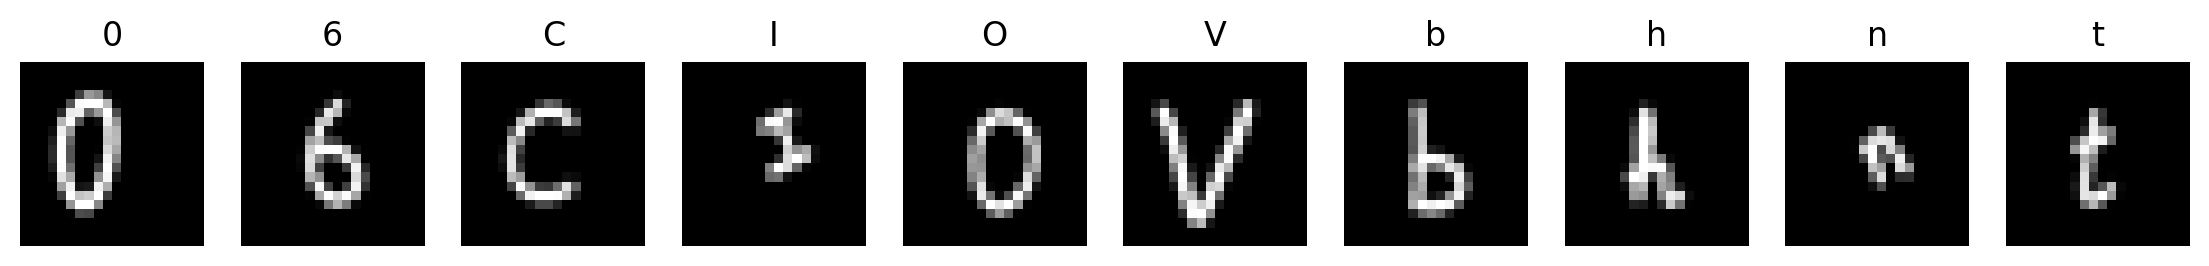
\includegraphics[width=\linewidth]{figures/sample_images.png}
\caption{Ten sample images after grayscale conversion, resizing to 20$\times$20 and inversion.}
\label{fig:samples}
\end{figure}

\textbf{Inference:}
The same kind of character is drawn at very different sizes and stroke widths; for example the ``I'' and the ``n'' above are small, while the ``0'' and ``O'' fill most of the box. The pen stroke covers only the middle part of the 20$\times$20 grid, so each character is described by a small number of active pixels. Shapes such as ``0'' and ``O'' look almost the same, which suggests that some classes will be hard to separate.

\subsection{Statistical Summary}
Table~\ref*{tab:stats} summarises all $3410\times400$ pixel values after scaling to $[0,1]$.

\begin{table}[H]
\centering
\begin{tabular}{lc}
\toprule
Statistic & Value \\
\midrule
Count & 1,364,000 \\
Mean & 0.060 \\
Standard deviation & 0.199 \\
Minimum & 0.000 \\
25\% / 50\% / 75\% & 0.000 / 0.000 / 0.000 \\
Maximum & 1.000 \\
Share of stroke pixels ($>0.5$) & 5.9\% \\
\bottomrule
\end{tabular}
\caption{Statistical summary of the pixel values.}
\label{tab:stats}
\end{table}

Even the 75th percentile is zero, so at least three quarters of all pixel values are background.

\subsection{Missing Value Analysis}
Both the label file and the pixel matrix were checked. There are no missing labels or image paths and no missing pixel values (0 in both cases), so no imputation was needed.

\subsection{Class Distribution}
\begin{figure}[H]
\centering
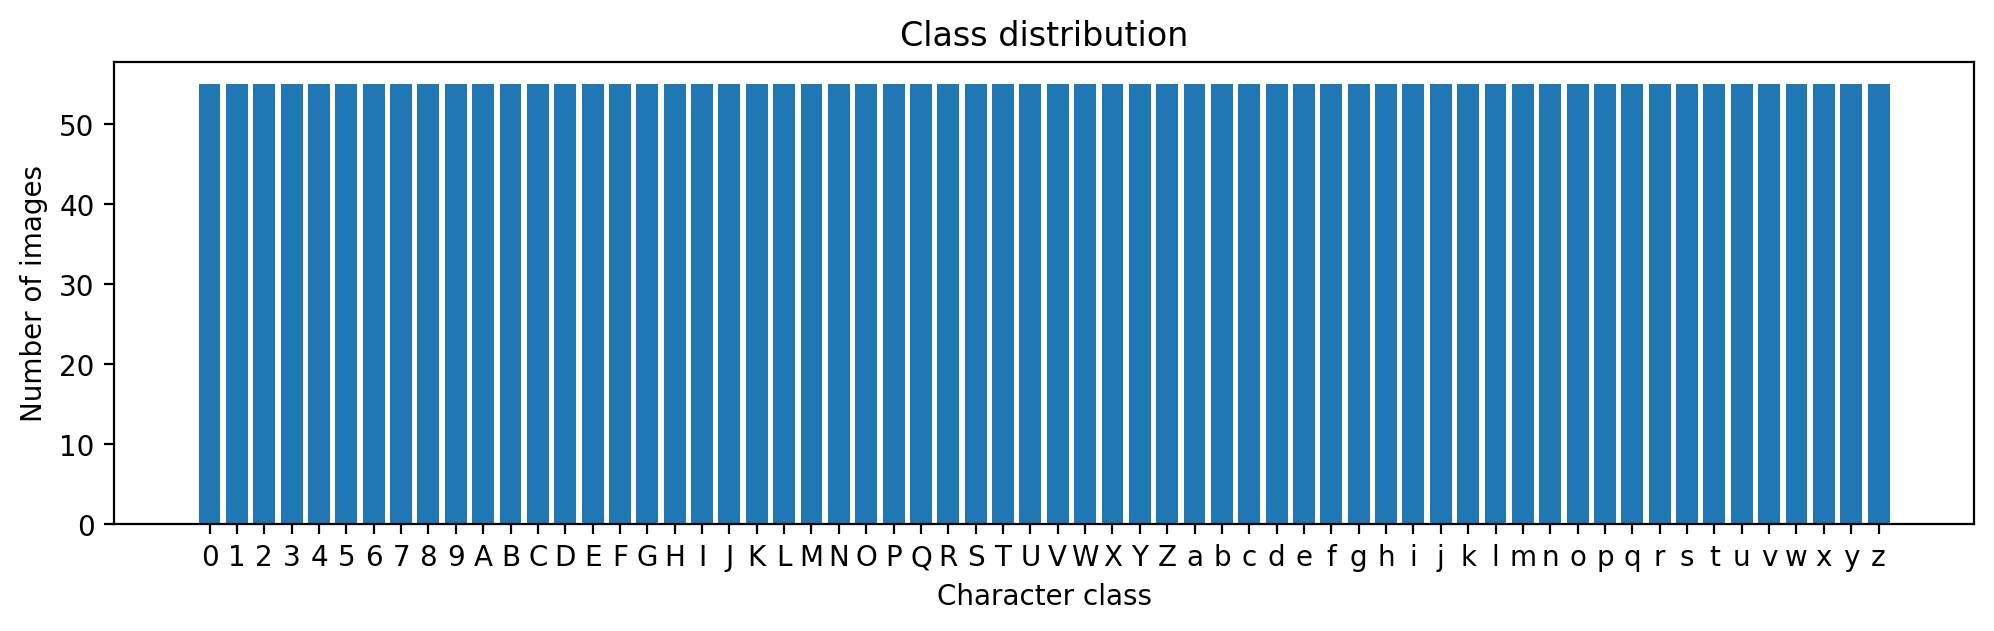
\includegraphics[width=0.95\linewidth]{figures/class_distribution.png}
\caption{Number of images in each of the 62 classes.}
\label{fig:classdist}
\end{figure}

\textbf{Inference:}
Every class has exactly 55 images, so the dataset is perfectly balanced. Accuracy is therefore a fair metric here and no resampling is needed. Random guessing would give only about 1.6\% accuracy (1/62). With a stratified split, each class has 11 test images, so the accuracy of a single class can only change in steps of about 9\%.

\subsection{Correlation Matrix}
\begin{figure}[H]
\centering
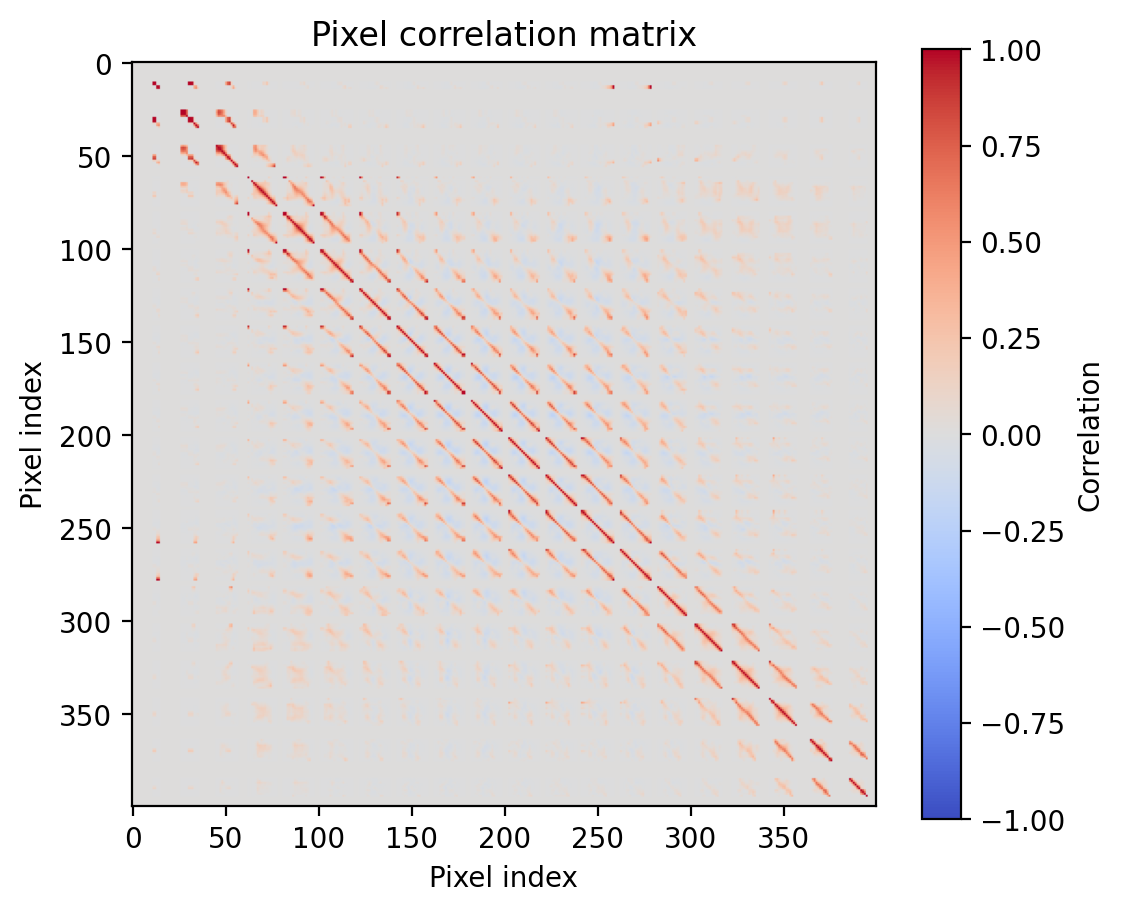
\includegraphics[width=0.65\linewidth]{figures/correlation_matrix.png}
\caption{Correlation matrix of the 400 pixel features.}
\label{fig:corr}
\end{figure}

\textbf{Inference:}
Most pixel pairs have a correlation close to zero (grey area). The strong values lie on a thin diagonal band, which means a pixel is mostly related to its immediate neighbours along the stroke. The same band repeats every 20 indices, which is the neighbouring row of the image. Strong negative correlations are almost absent. No small group of pixels is enough to identify a character, so the classifier has to combine many pixels.

\subsection{Feature Distribution}
\begin{figure}[H]
\centering
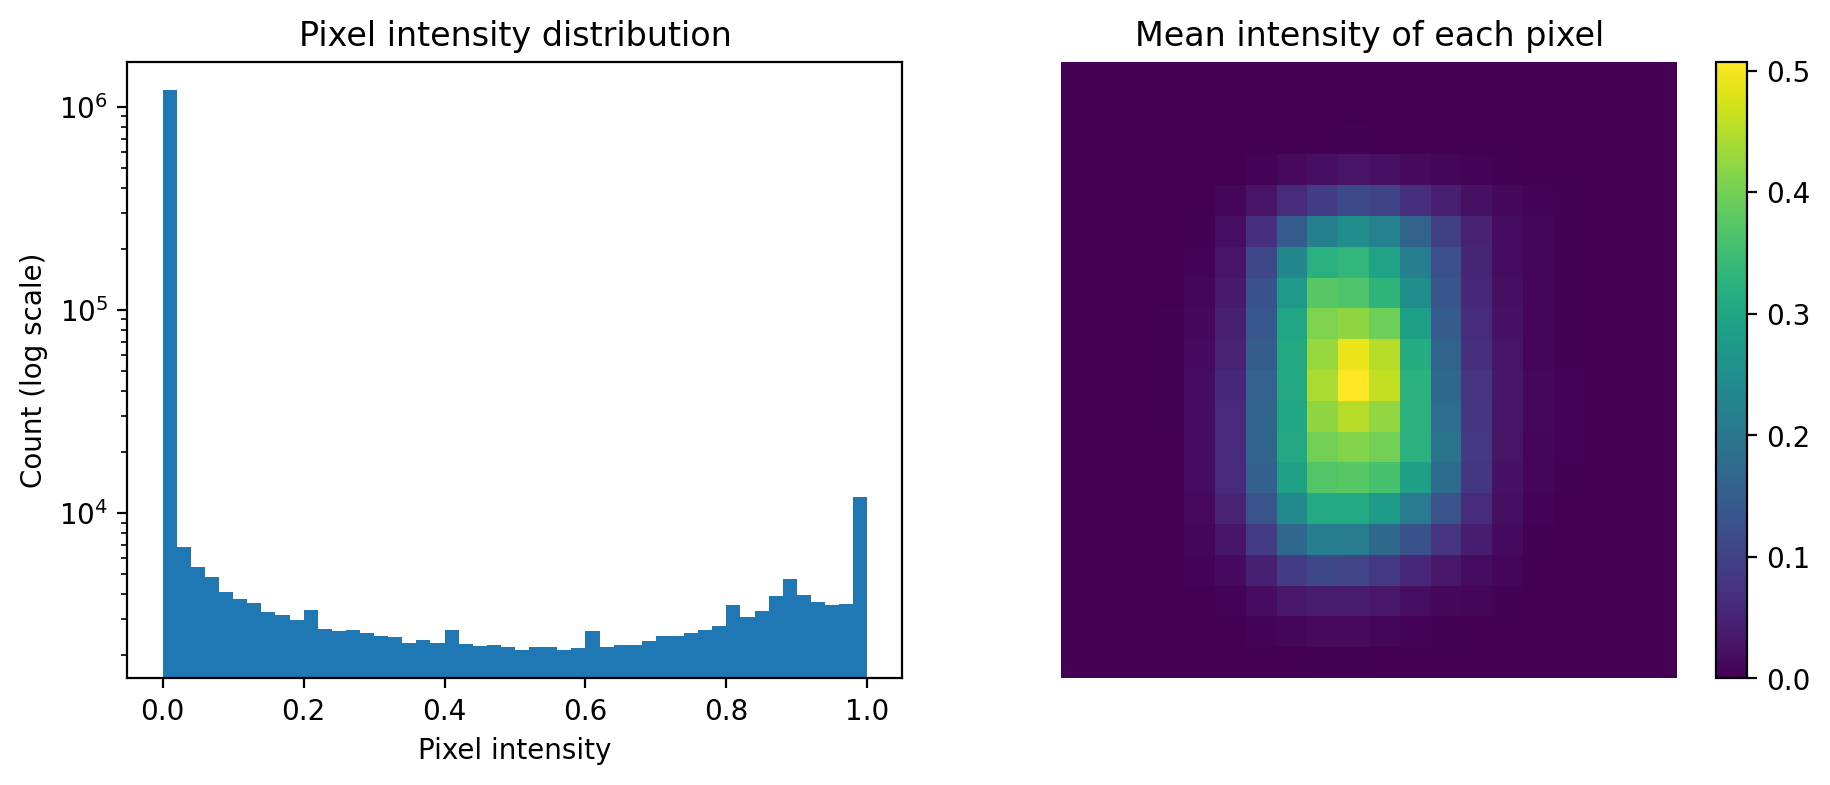
\includegraphics[width=\linewidth]{figures/feature_distribution.png}
\caption{Left: histogram of all pixel values (log scale). Right: mean intensity of each pixel over the whole dataset.}
\label{fig:featdist}
\end{figure}

\textbf{Inference:}
The histogram has a very large peak at 0 (background) and a smaller peak at 1 (centre of the pen stroke); the values in between come from the smoothing done by resizing. The mean image is bright only in the central region, and the outer border is almost always zero. Border pixels therefore carry almost no information, and they also appear as empty rows and columns in the correlation matrix.

% ------------------------------------------------------------
\section{Data Preprocessing}
\begin{itemize}
\item \textbf{Missing value handling:} not required, as no value is missing.
\item \textbf{Encoding:} the 62 character labels were converted to integers 0--61. For the PLA targets and for the ROC and precision-recall curves, the labels were also converted to one-hot vectors.
\item \textbf{Feature scaling:} each image is converted to grayscale, inverted (stroke = 1, background = 0) and divided by 255, so all values lie in $[0,1]$.
\item \textbf{Train-test split:} stratified 80/20 split (2,728 / 682 images). The training part was split again 80/20 (2,182 / 546) to get a validation set for tuning. The test set was used only once, for the final comparison.
\item \textbf{Feature engineering:} images were resized to 20$\times$20 and flattened into 400 features. No other features were created.
\end{itemize}

% ------------------------------------------------------------
\section{Machine Learning Algorithm}

\subsection{Model A: Perceptron Learning Algorithm (PLA)}
\textbf{Working principle.} The perceptron \cite{rosenblatt} computes a weighted sum of the inputs and passes it through a step function. Because there are 62 classes, one perceptron is used per class (one-vs-rest), giving 62 output neurons. During training, the samples are visited one by one in random order and the weights change only when a neuron gives a wrong output. At prediction time, the class whose neuron has the largest net input is selected.

\textbf{Mathematical formulation.} For class $k$ and input $\mathbf{x}$,
\begin{equation}
z_k = \mathbf{w}_k^{\top}\mathbf{x} + b_k, \qquad \hat{y}_k = \begin{cases} 1 & z_k \ge 0 \\ 0 & z_k < 0 \end{cases}
\end{equation}
\begin{equation}
\mathbf{w}_k \leftarrow \mathbf{w}_k + \eta\,(y_k-\hat{y}_k)\,\mathbf{x}, \qquad b_k \leftarrow b_k + \eta\,(y_k-\hat{y}_k), \qquad \hat{c} = \arg\max_k z_k
\end{equation}
where $y_k=1$ for the true class and 0 otherwise, and $\eta$ is the learning rate.

\textbf{Advantages.} It is simple, very fast to train, needs no derivatives, and is easy to explain.

\textbf{Limitations.} It can only draw linear boundaries, so it converges only when the classes are linearly separable. Its output is a hard 0/1 value, so it gives no class probabilities.

\subsection{Model B: Multilayer Perceptron (MLP)}
\textbf{Working principle.} An MLP has an input layer, one or more hidden layers with a non-linear activation, and an output layer. The hidden layers build new features from the pixels, which lets the network learn non-linear decision boundaries. The weights are learned by backpropagation \cite{rumelhart}, which sends the error backwards through the layers and updates the weights by gradient descent \cite{goodfellow}.

\textbf{Mathematical formulation.} For layer $l$ with weights $W^{(l)}$ and bias $\mathbf{b}^{(l)}$,
\begin{equation}
\mathbf{a}^{(l)} = \varphi\!\left(W^{(l)}\mathbf{a}^{(l-1)} + \mathbf{b}^{(l)}\right), \qquad p_k = \frac{e^{z_k}}{\sum_{j=1}^{62} e^{z_j}}
\end{equation}
where $\varphi$ is ReLU, tanh or sigmoid, and the output layer uses softmax. The cost function is the cross-entropy over $N$ training samples,
\begin{equation}
L = -\frac{1}{N}\sum_{i=1}^{N}\sum_{k=1}^{62} y_{ik}\log p_{ik}.
\end{equation}
With softmax and cross-entropy the output error is $\boldsymbol{\delta}^{(L)}=\mathbf{p}-\mathbf{y}$, and it is propagated backwards as $\boldsymbol{\delta}^{(l)}=\big(W^{(l+1)\top}\boldsymbol{\delta}^{(l+1)}\big)\odot\varphi'(\mathbf{z}^{(l)})$. The gradient of the weights is $\partial L/\partial W^{(l)}=\boldsymbol{\delta}^{(l)}\mathbf{a}^{(l-1)\top}$. SGD updates a weight as $\theta\leftarrow\theta-\eta\,\nabla_\theta L$, whereas Adam \cite{adam} keeps running averages of the gradient and its square and scales the step for every weight.

\textbf{Advantages.} It learns non-linear patterns, gives class probabilities, and works with different activations, optimizers and depths.

\textbf{Limitations.} It has many hyperparameters to tune, needs more computation than PLA, and overfits easily when the training set is small.

% ------------------------------------------------------------
\section{Experimental Setup}
\begin{table}[H]
\centering
\begin{tabular}{ll}
\toprule
Python Version & 3.12.3 \\
Scikit-Learn Version & 1.8.0 \cite{sklearn} \\
IDE & Jupyter Notebook \\
Operating System & Ubuntu 24.04 LTS (Linux) \\
Hardware & Intel Xeon @ 2.10 GHz, 1 vCPU, 3 GB RAM \\
\bottomrule
\end{tabular}
\end{table}
The complete notebook (loading the images, tuning 108 MLP configurations, final training and all plots) runs in about five minutes on this hardware.

% ------------------------------------------------------------
\section{Hyperparameter Selection}

\subsection{PLA}
\begin{table}[H]
\centering
\begin{tabular}{ll}
\toprule
Parameter & Value\\
\midrule
Activation & Step (threshold at 0) \\
Learning rate $\eta$ & 0.1 \\
Epochs & 30 \\
Initial weights and bias & 0 \\
Sample order & Shuffled in every epoch \\
\bottomrule
\end{tabular}
\end{table}
With zero initial weights, $\eta$ only rescales the weights and does not change the sign of $z_k$, so the value of $\eta$ has no effect on the PLA result.

\subsection{MLP: Search Space}
Every combination in Table~\ref*{tab:grid} (3$\times$2$\times$3$\times$2$\times$3 = 108 runs) was trained for 50 epochs on the train part and scored on the validation part. The last column gives the mean validation accuracy over all runs that use that value.

\begin{table}[H]
\centering
\begin{tabular}{lp{7.5cm}l}
\toprule
Hyperparameter & Values tried (mean validation accuracy) & Chosen \\
\midrule
Activation & ReLU (0.321), Tanh (0.327), Sigmoid (0.192) & ReLU \\
Optimizer & SGD (0.259), Adam (0.301) & Adam \\
Learning rate & 0.001 (0.246), 0.01 (0.372), 0.1 (0.222) & 0.01 \\
Batch size & 32 (0.298), 128 (0.262) & 128 \\
Hidden layers & 1: (128) (0.329), 2: (128, 64) (0.273), 3: (128, 64, 32) (0.238) & (128, 64) \\
\bottomrule
\end{tabular}
\caption{Search space, mean validation accuracy per value, and the chosen value.}
\label{tab:grid}
\end{table}

SGD was run with scikit-learn's default momentum of 0.9 (Nesterov), and Adam with its default $\beta_1=0.9$ and $\beta_2=0.999$. The impact of a hyperparameter was measured as the difference between the best and worst mean accuracy of its values: learning rate 0.151, activation 0.135, hidden layers 0.092, optimizer 0.043 and batch size 0.036.

\subsection{MLP: Best Configurations}
\begin{table}[H]
\centering
\begin{tabular}{clllccc}
\toprule
Rank & Activation & Optimizer & LR & Batch & Hidden layers & Val.\ acc. \\
\midrule
1 & ReLU & Adam & 0.01 & 128 & (128, 64) & 0.518 \\
2 & ReLU & SGD & 0.1 & 32 & (128) & 0.509 \\
3 & Sigmoid & Adam & 0.01 & 128 & (128, 64) & 0.505 \\
4 & ReLU & SGD & 0.01 & 32 & (128, 64, 32) & 0.502 \\
5 & ReLU & SGD & 0.1 & 128 & (128, 64) & 0.498 \\
\bottomrule
\end{tabular}
\caption{Five best configurations on the validation set.}
\end{table}

\subsection{MLP: Final Choice and Justification}
\begin{table}[H]
\centering
\begin{tabular}{ll}
\toprule
Parameter & Value\\
\midrule
Hidden layers & 2 layers, 128 and 64 neurons \\
Activation & ReLU \\
Optimizer & Adam \\
Learning rate & 0.01 \\
Batch size & 128 \\
Cost function & Cross-entropy \\
Epochs & 50 \\
L2 penalty ($\alpha$) & 0.0001 (scikit-learn default) \\
\bottomrule
\end{tabular}
\end{table}

\begin{itemize}
\item \textbf{Activation:} ReLU gave the best individual configurations. Tanh has a similar average, but Sigmoid is clearly worse (0.192), probably because its gradients become very small.
\item \textbf{Optimizer:} Adam has the best single result and a higher average than SGD, since it adapts its step size and is less sensitive to the learning rate.
\item \textbf{Learning rate:} 0.01 has the best average (0.372). At 0.001 training is too slow for 50 epochs, and at 0.1 the average falls to 0.222 because only some SGD runs still do well.
\item \textbf{Batch size:} the effect is small (0.036). 128 was kept because it belongs to the best run and makes each epoch faster.
\item \textbf{Hidden layers:} the best 1-, 2- and 3-layer networks score 0.509, 0.518 and 0.502, so depth hardly matters. Two layers gave the top score.
\item \textbf{Cost function:} training the best configuration with mean squared error (an \texttt{MLPRegressor} on one-hot targets) gave only 0.075 validation accuracy, against 0.518 with cross-entropy. With 62 mostly-zero targets, the MSE gradients are very small and the network learns slowly.
\end{itemize}

% ------------------------------------------------------------
\section{Results}
The final PLA and MLP were trained on the full training part (2,728 images) and evaluated on the 682 test images. An MLP with the untuned scikit-learn defaults is included to show the effect of tuning. Precision, recall, F1-score and ROC-AUC are macro averages over the 62 classes.

\begin{table}[H]
\centering
\begin{tabular}{lccc}
\toprule
Metric & PLA & MLP (default) & MLP (tuned)\\
\midrule
Accuracy & 0.232 & 0.424 & 0.529 \\
Precision & 0.263 & 0.433 & 0.549 \\
Recall & 0.232 & 0.424 & 0.529 \\
F1-score & 0.209 & 0.418 & 0.531 \\
ROC-AUC & 0.825 & 0.912 & 0.954 \\
\midrule
Training accuracy & 0.489 & 0.644 & 0.999 \\
\bottomrule
\end{tabular}
\caption{Test-set results of the three models.}
\end{table}

% ------------------------------------------------------------
\section{Result Visualization}
The class distribution and correlation matrix are shown in Figures~\ref*{fig:classdist} and~\ref*{fig:corr} (Section 4). The remaining graphs of the experiment follow.

\subsection{Confusion Matrices}
\begin{figure}[H]
\centering
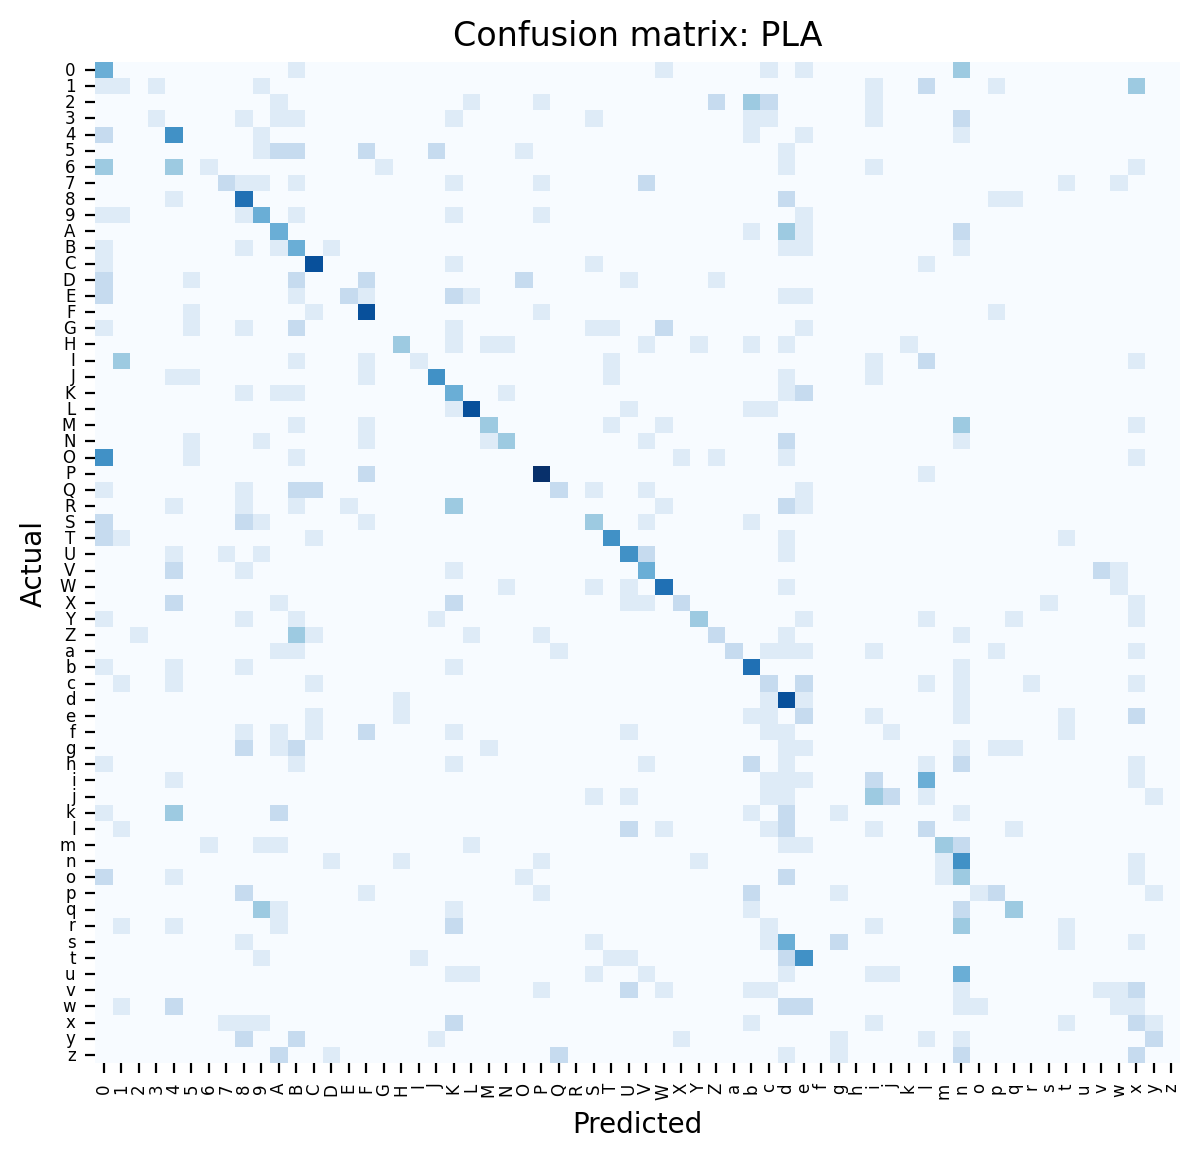
\includegraphics[width=\linewidth]{figures/confusion_pla.png}
\caption{Confusion matrix of the PLA on the test set.}
\label{fig:cmpla}
\end{figure}

\textbf{Inference:}
The diagonal of the PLA matrix is weak and the errors are spread over the whole matrix. A few classes attract far too many predictions: ``d'' is predicted 51 times, ``n'' 46 times, ``0'' 34 times and ``B'' 32 times, although every class has only 11 test images. Five classes are never predicted at all. The best class is ``P'' with 73\% recall.

\begin{figure}[H]
\centering
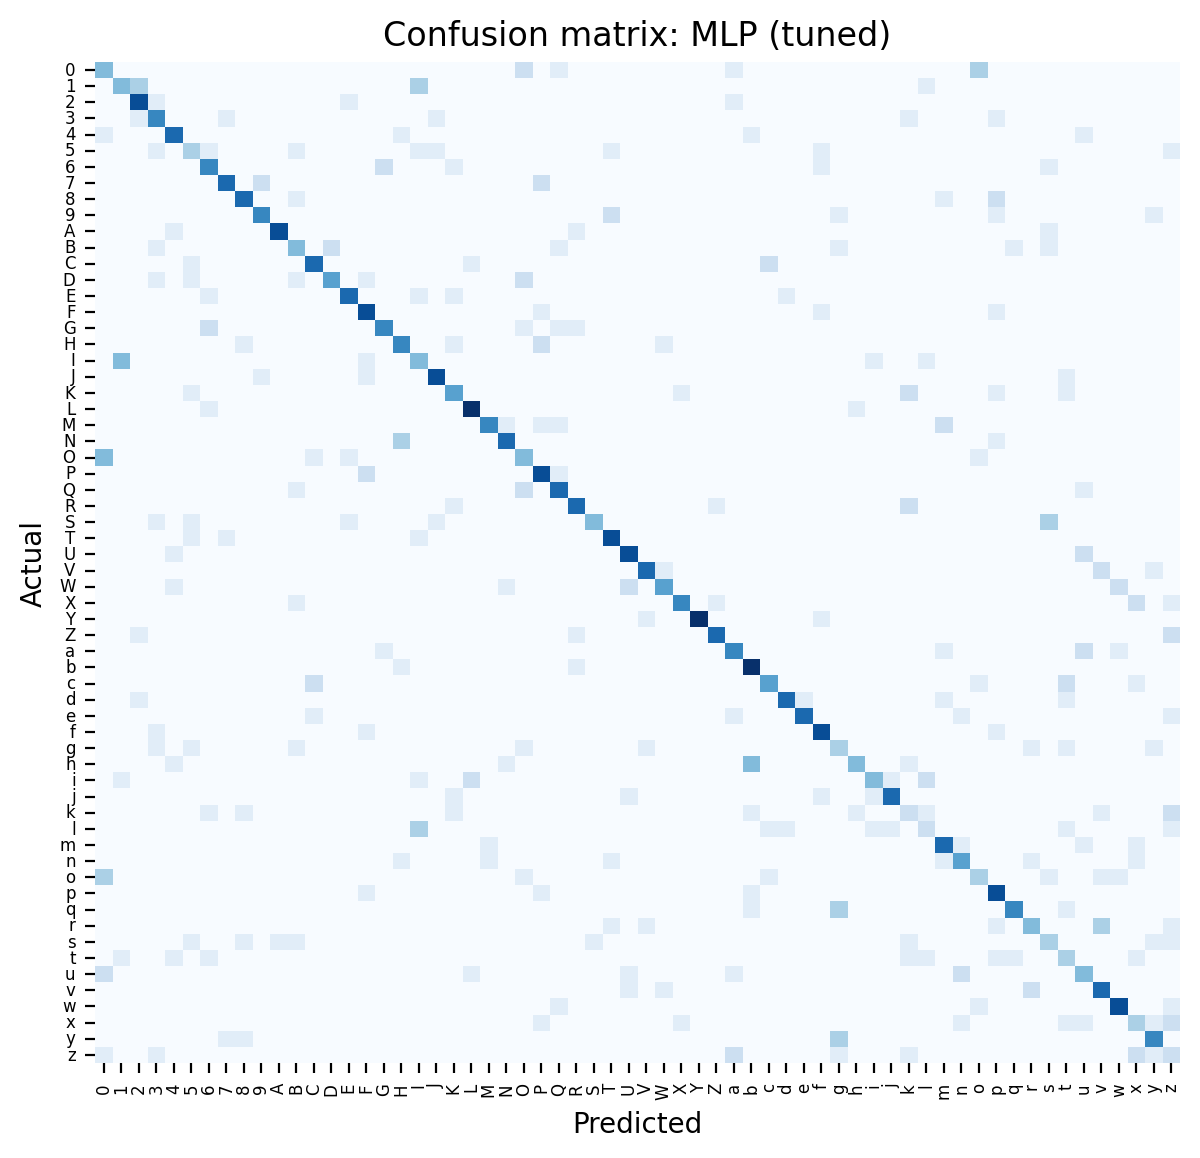
\includegraphics[width=\linewidth]{figures/confusion_mlp.png}
\caption{Confusion matrix of the tuned MLP on the test set.}
\label{fig:cmmlp}
\end{figure}

\textbf{Inference:}
The tuned MLP shows a clear diagonal, with 361 of 682 test images classified correctly. ``L'', ``Y'' and ``b'' are recognised best (82\%), and ``k'', ``z'' and ``l'' worst (18\%). The most common mistakes are between look-alike shapes: ``I'' and ``1'', ``O'' and ``0'', ``h'' and ``b'', ``q'' and ``g''. Of the 321 wrong predictions, 33 are the same letter in the wrong case.

\subsection{ROC Curves}
\begin{figure}[H]
\centering
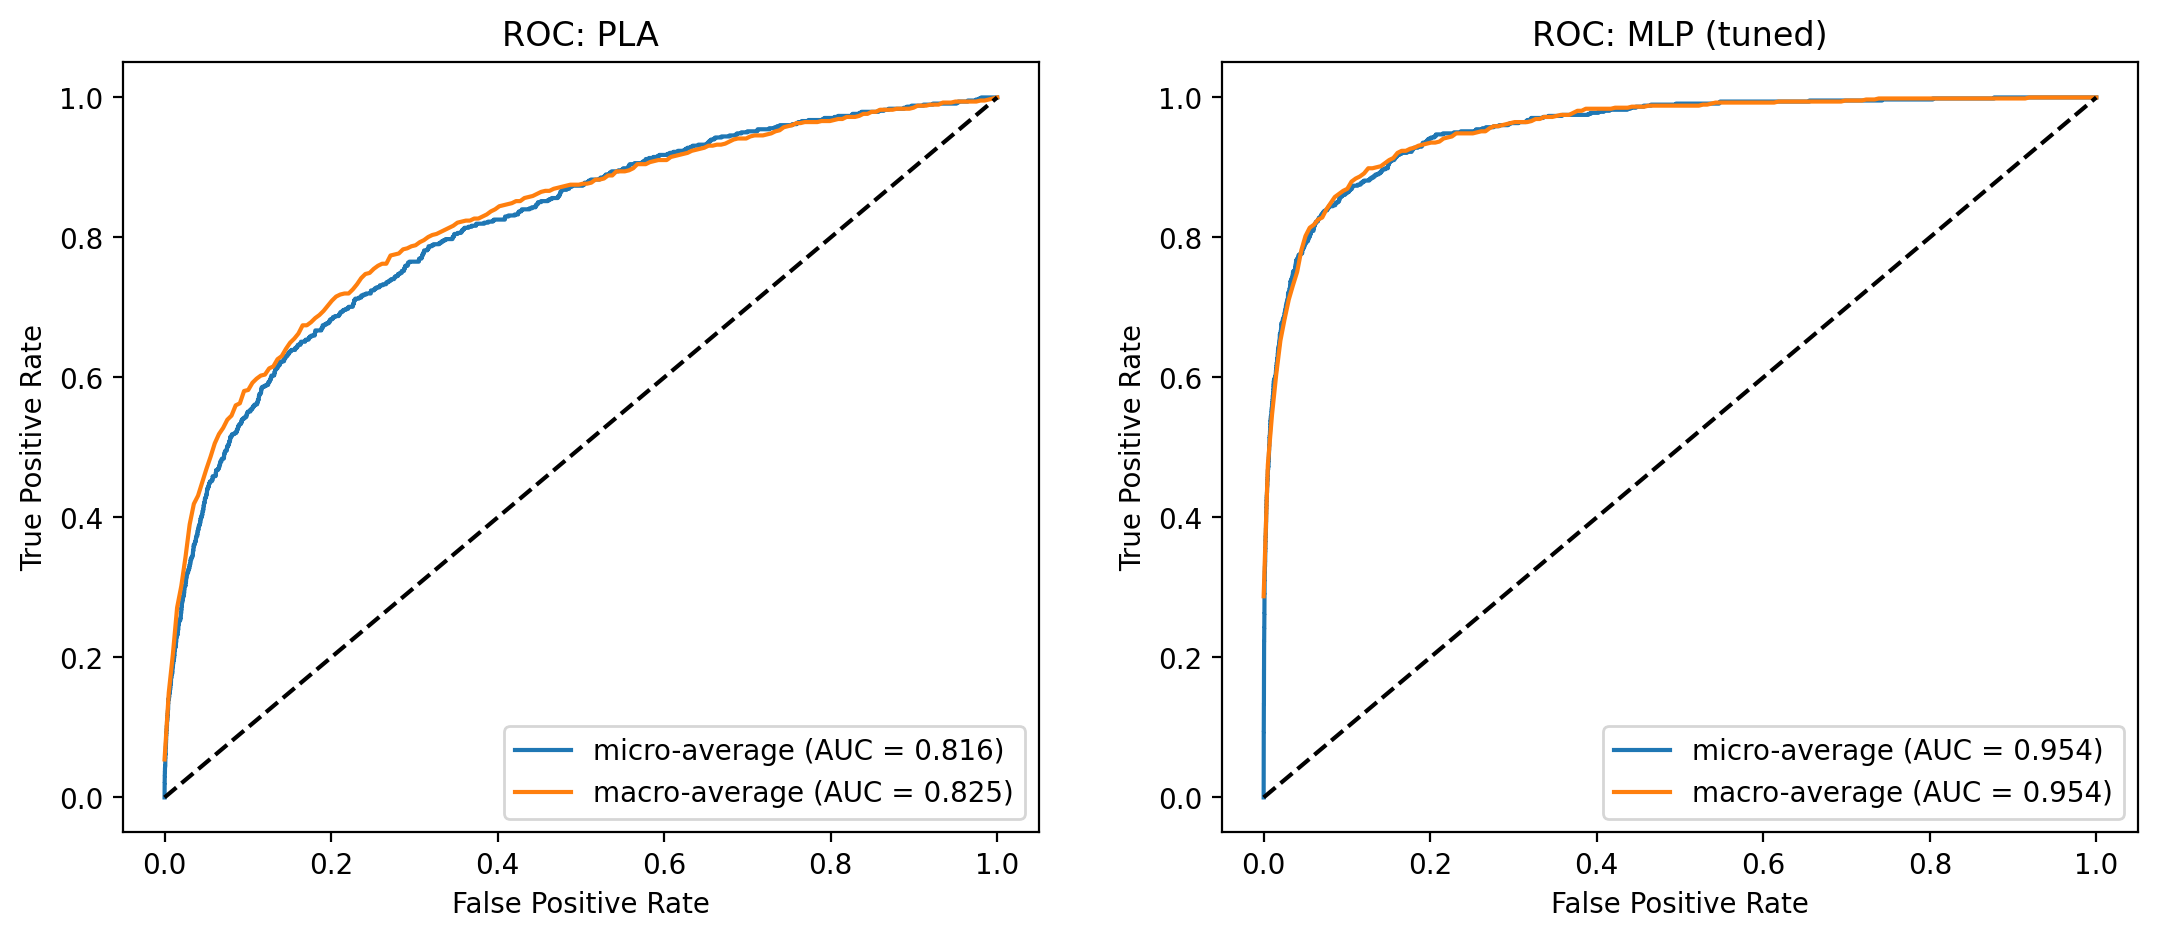
\includegraphics[width=\linewidth]{figures/roc_curves.png}
\caption{Micro- and macro-average ROC curves (one-vs-rest) of the PLA and the tuned MLP.}
\label{fig:roc}
\end{figure}

\textbf{Inference:}
The macro-average AUC is 0.825 for the PLA and 0.954 for the MLP (micro-average: 0.816 and 0.954). The PLA curve lies above the diagonal, so its scores still rank the correct class better than chance, but it rises slowly. The MLP reaches a true positive rate of about 0.8 at a false positive rate of about 0.05. The AUC is high even though accuracy is only 53\% because each one-vs-rest problem has 61 negative classes and the AUC measures ranking, not the top-1 decision.

\subsection{Precision-Recall Curves}
\begin{figure}[H]
\centering
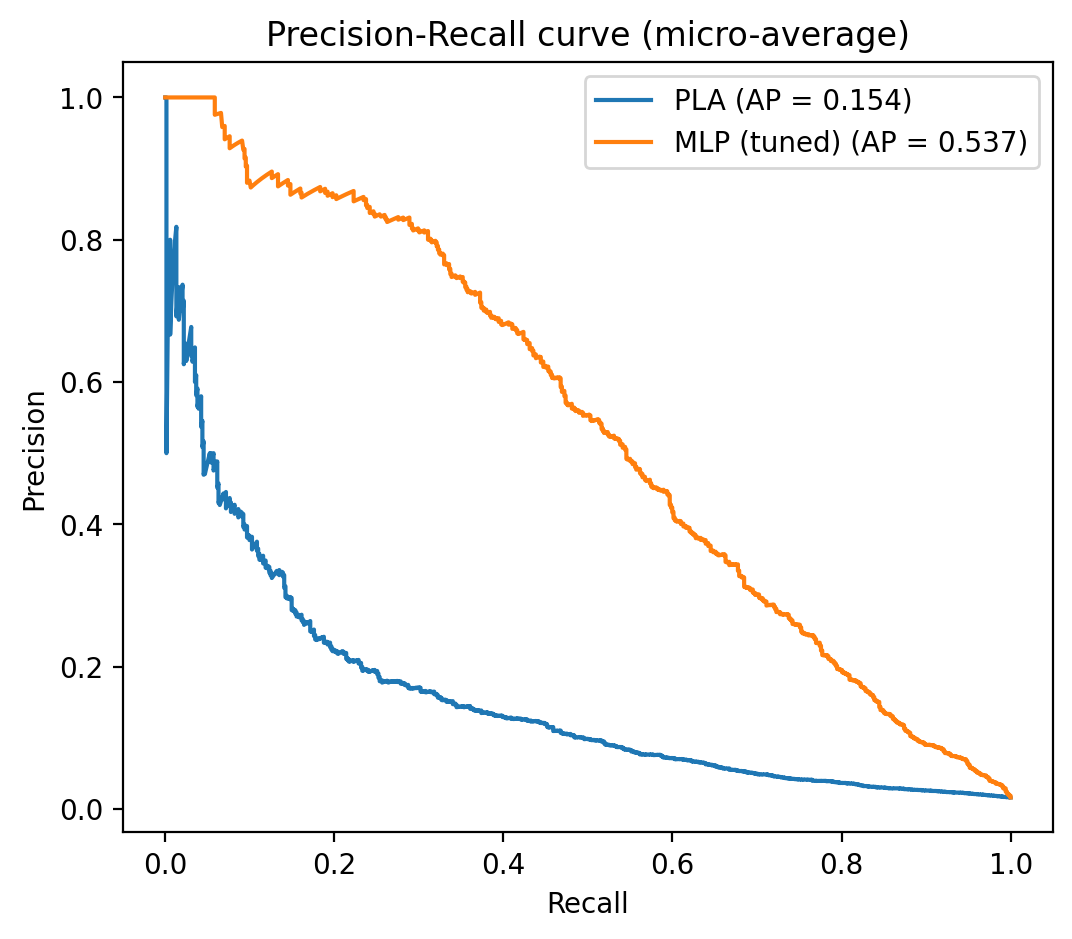
\includegraphics[width=0.6\linewidth]{figures/pr_curves.png}
\caption{Micro-average precision-recall curves of the PLA and the tuned MLP.}
\label{fig:pr}
\end{figure}

\textbf{Inference:}
The average precision is 0.537 for the MLP and only 0.154 for the PLA; a random scorer would get about 0.016. The MLP holds a precision near or above 0.8 until a recall of about 0.3 and then falls slowly. The PLA drops below 0.5 at a recall of less than 0.05. Since the PLA output is a raw net input and not a probability, its curve is also less smooth.

\subsection{Learning Curves (Training Error vs Epochs)}
\begin{figure}[H]
\centering
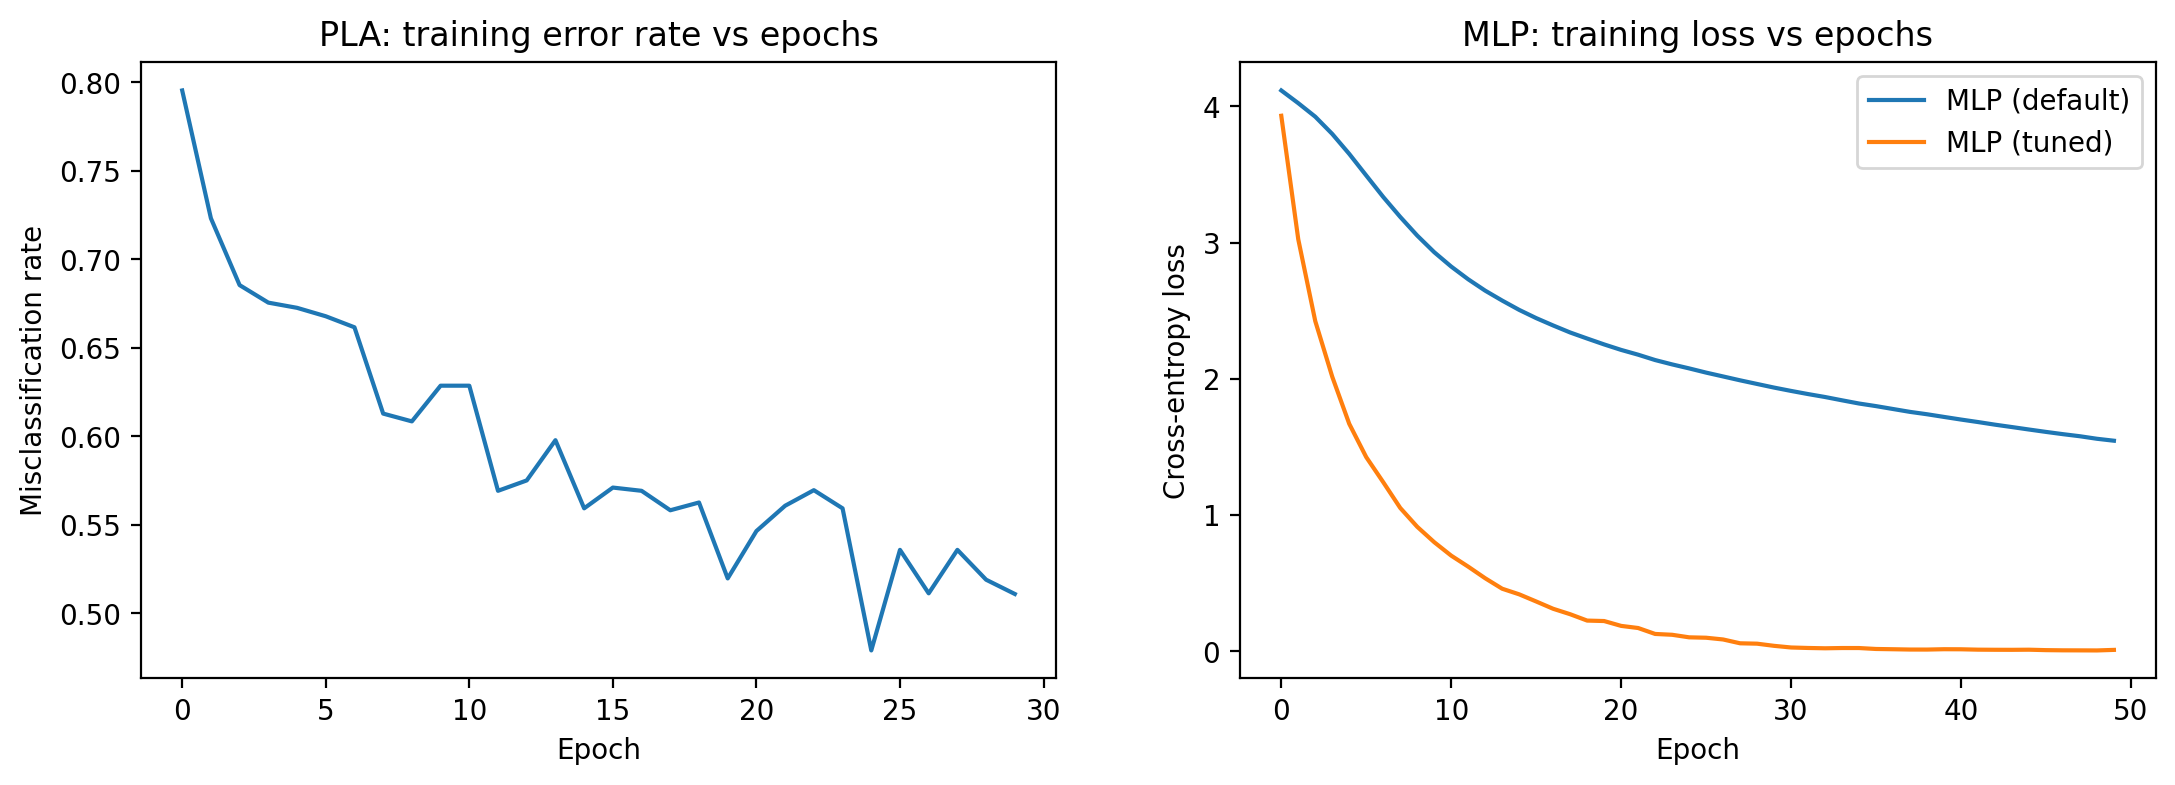
\includegraphics[width=\linewidth]{figures/training_curves.png}
\caption{Left: PLA training error rate per epoch. Right: cross-entropy training loss of the default and tuned MLP.}
\label{fig:curves}
\end{figure}

\textbf{Inference:}
The PLA error falls from 0.80 to about 0.51 in 30 epochs, with a lowest value of 0.48 near epoch 25, and it keeps jumping up and down instead of settling. This is what we expect when the classes are not linearly separable. The default MLP loss goes from 4.12 to 1.55 and is still falling after 50 epochs. The tuned MLP goes from 3.93 to 0.011 and is below 0.1 by about epoch 25, so tuning made the training much faster.

\subsection{SGD vs Adam}
\begin{figure}[H]
\centering
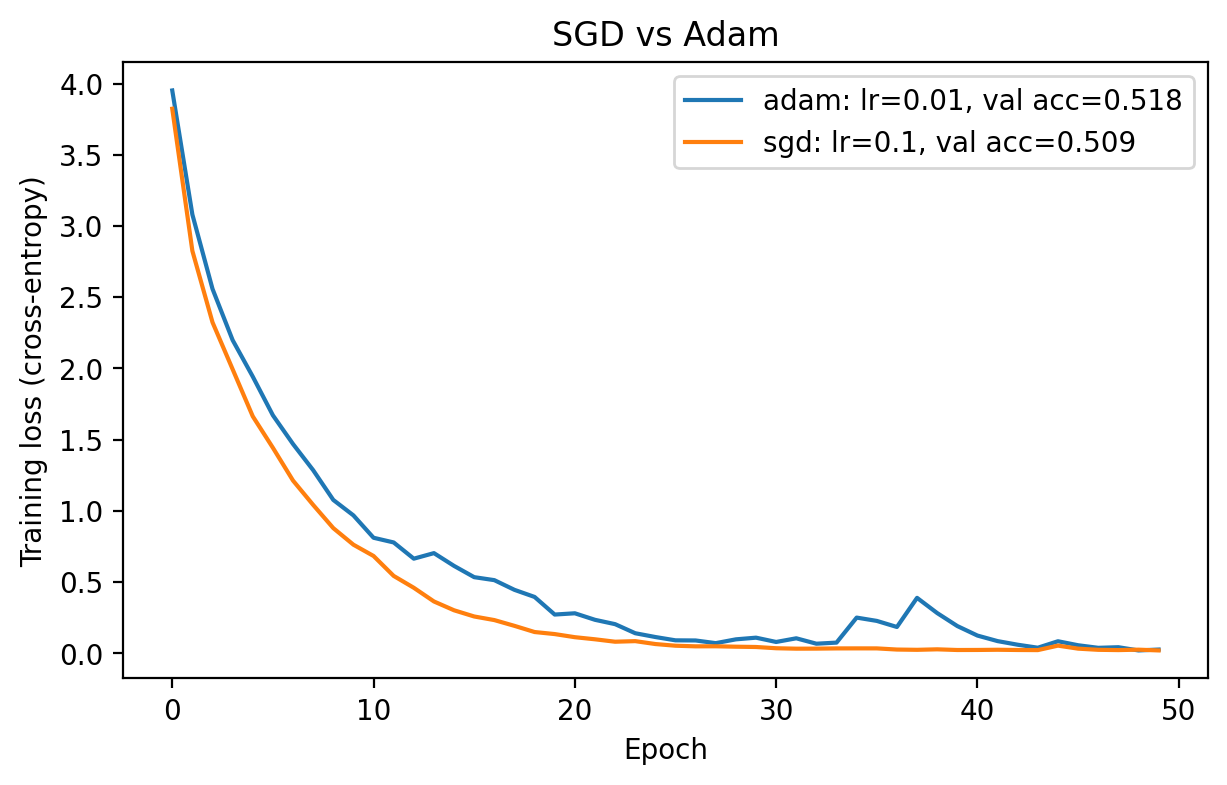
\includegraphics[width=0.65\linewidth]{figures/sgd_vs_adam.png}
\caption{Training loss of the best SGD run and the best Adam run.}
\label{fig:optim}
\end{figure}

\textbf{Inference:}
The best Adam run (learning rate 0.01, batch 128) reached 0.518 validation accuracy and the best SGD run (learning rate 0.1, batch 32) reached 0.509, a gap of about five images out of 546. SGD falls faster at the start, partly because batch size 32 gives four times more updates per epoch. The Adam curve shows a small bump around epochs 35--40 before it recovers. Both losses end close to zero.

\subsection{Feature Importance}
Feature importance is not applicable here. Neither the PLA nor scikit-learn's MLP provides a built-in importance score, and the inputs are raw pixels, so no individual pixel has a meaning of its own.

% ------------------------------------------------------------
\section{Discussion}

\subsection{PLA vs MLP}
\begin{table}[H]
\centering
\begin{tabular}{p{3.2cm}p{5.7cm}p{5.7cm}}
\toprule
Aspect & PLA & MLP (tuned) \\
\midrule
Boundary & Linear only & Non-linear \\
Test accuracy / F1 & 23.2\% / 0.209 & 52.9\% / 0.531 \\
Convergence & Error keeps fluctuating around 50\% & Loss reaches almost 0 in about 30 epochs \\
Strengths & Simple, fast, easy to explain & Learns complex shapes, gives probabilities \\
Weaknesses & Fails on non-separable classes, no probabilities & Needs tuning, more computation, overfits \\
\bottomrule
\end{tabular}
\end{table}
Tuning also helped: the untuned MLP reached 42.4\% test accuracy and the tuned one 52.9\%, an increase of about 10 points, with much faster convergence.

\subsection{Observation Questions}
\textbf{Why does PLA underperform compared to MLP?}
Characters from 62 classes are not linearly separable in pixel space, and the PLA can only place one straight boundary per class. Its training error never goes to zero (training accuracy 48.9\%) because later updates undo earlier ones. The hidden layers of the MLP combine pixels into strokes and curves, which allows curved boundaries.

\textbf{Which hyperparameters had the most impact?}
The learning rate (0.151) and the activation function (0.135) had the largest effect, followed by the number of hidden layers (0.092). The optimizer (0.043) and batch size (0.036) changed the result much less.

\textbf{Did optimizer choice (SGD vs Adam) affect convergence?}
Adam was better on average (0.301 against 0.259) since it works over a wider range of learning rates, while SGD was too slow at 0.001. With a well-chosen rate of 0.1, SGD reached almost the same accuracy (0.509 against 0.518) and converged as quickly. The optimizer therefore matters mainly through its sensitivity to the learning rate.

\textbf{Did more hidden layers always improve results?}
No. The mean validation accuracy dropped from 0.329 to 0.273 to 0.238 for one, two and three layers, and the best network of each depth scored almost the same (0.509, 0.518, 0.502). With only about 44 training images per class, deeper networks have more weights to fit, are harder to train in 50 epochs and overfit more.

\textbf{Did the MLP overfit? How can it be reduced?}
Yes. The tuned MLP has 99.9\% training accuracy but 52.9\% test accuracy, and its training loss goes to zero while validation accuracy stays flat. Overfitting can be reduced with L2 regularization (larger $\alpha$), early stopping, dropout, a smaller network, and above all more data or data augmentation such as small shifts, rotations and stroke-width changes.

\subsection{Limitations and Improvements}
The dataset is small (55 images per class), so the gap between training and test accuracy is large. The 20$\times$20 raw pixels are also a weak representation, since the characters occupy only the centre of the image. The validation set has 546 images, so differences of one or two percentage points between configurations are within noise, and only a single split was used. The MSE comparison used a regressor with a linear output layer, so it is not an exact swap of the loss alone. Possible improvements are data augmentation, cross-validation, regularization with early stopping, better features such as HOG, and a convolutional network, which suits image data better than a fully connected one.

% ------------------------------------------------------------
\section{Conclusion}
A one-vs-rest PLA and a tuned MLP were compared on 3,410 handwritten character images from 62 classes. The PLA reached 23.2\% test accuracy (macro F1 0.209, ROC-AUC 0.825) and its training error never converged, which shows that the classes are not linearly separable. The best MLP (ReLU, Adam, learning rate 0.01, batch size 128, hidden layers 128 and 64, cross-entropy loss) reached 52.9\% accuracy (macro F1 0.531, ROC-AUC 0.954), and tuning gave about 10 points over the default MLP. Learning rate and activation function mattered most, while extra hidden layers gave no gain. The large gap between training accuracy (99.9\%) and test accuracy shows that overfitting is the main remaining problem, which more data or augmentation should address.

% ------------------------------------------------------------
\section{References}
\begin{thebibliography}{9}
\bibitem{rosenblatt} F. Rosenblatt, ``The perceptron: A probabilistic model for information storage and organization in the brain,'' \textit{Psychological Review}, vol. 65, no. 6, pp. 386--408, 1958.
\bibitem{rumelhart} D. E. Rumelhart, G. E. Hinton, and R. J. Williams, ``Learning representations by back-propagating errors,'' \textit{Nature}, vol. 323, no. 6088, pp. 533--536, 1986.
\bibitem{adam} D. P. Kingma and J. Ba, ``Adam: A method for stochastic optimization,'' in \textit{Proc. 3rd Int. Conf. Learning Representations (ICLR)}, San Diego, CA, USA, 2015.
\bibitem{goodfellow} I. Goodfellow, Y. Bengio, and A. Courville, \textit{Deep Learning}. Cambridge, MA, USA: MIT Press, 2016.
\bibitem{sklearn} F. Pedregosa \textit{et al.}, ``Scikit-learn: Machine learning in Python,'' \textit{J. Mach. Learn. Res.}, vol. 12, pp. 2825--2830, 2011.
\bibitem{decampos} T. E. de Campos, B. R. Babu, and M. Varma, ``Character recognition in natural images,'' in \textit{Proc. Int. Conf. Computer Vision Theory and Applications (VISAPP)}, Lisbon, Portugal, Feb. 2009.
\bibitem{kaggle} D. Dave, ``English handwritten characters dataset,'' Kaggle. [Online]. Available: \url{https://www.kaggle.com/datasets/dhruvildave/english-handwritten-characters-dataset}
\end{thebibliography}

\end{document}
